\setcounter{dang}{0}% \begin{name}
% 	{GV biên soạn: Nguyễn Hữu Cường\\ GV phản biện 1: Trung Anh\\ GV phản biện 2: Nguyễn Đức Lợi}
% 	{TOÁN 10-KNTT-CS}
% \end{name}
%----------------NỘI DUNG BIÊN SOẠN
\setcounter{section}{3}
\section{Phương trình quy về phương trình bậc hai}
%-------------------------------------------
\subsection{KIẾN THỨC TRỌNG TÂM}
\subsubsection{Phương trình dạng $\sqrt{ax^2+bx+c} = \sqrt{dx^2+ex+f}$}
\begin{boxdn}
		Để giải phương trình này, ta thực hiện các bước sau
\begin{itemize}
	\item \textbf{Bước 1:} Bình phương hai vế của phương trình để khử căn thức.
	\item \textbf{Bước 2:} Giải phương trình bậc hai nhận được sau khi bình phương $$ax^2+bx+c = dx^2+ex+f$$
	\item \textbf{Bước 3:} Thử lại và kết luận nghiệm.
\end{itemize}
\end{boxdn}
\subsubsection{Phương trình dạng $\sqrt{ax^2+bx+c} = dx+e$.}
\begin{boxdn}
		Các bước thực hiện tương tự như sau
\begin{itemize}
	\item \textbf{Bước 1:} Bình phương hai vế của phương trình để thu được một phương trình bậc hai $$ax^2+bx+c = (dx+e)^2.$$
	\item \textbf{Bước 2:} Giải phương trình bậc hai vừa nhận được.
	\item \textbf{Bước 3:} Thử lại và kết luận tập nghiệm.
\end{itemize}
\end{boxdn}
\subsection{PHÂN LOẠI VÀ PHƯƠNG PHÁP GIẢI TOÁN}
\begin{dang}{Phương trình dạng $\sqrt{ax^2+bx+c} = \sqrt{dx^2+ex+f}$}
	Để giải phương trình này, ta thực hiện các bước sau
	\begin{itemize}
		\item \textbf{Bước 1:} Bình phương hai vế của phương trình để khử căn thức.
		\item \textbf{Bước 2:} Giải phương trình bậc hai nhận được sau khi bình phương $$ax^2+bx+c = dx^2+ex+f$$
		\item \textbf{Bước 3:} Thử lại và kết luận nghiệm.
	\end{itemize}
\end{dang}
\begin{vd}
	Tìm tập nghiệm $S$ của phương trình $\sqrt{2x^2 - 5x - 9} = \sqrt{x^2 - 2x - 5}$.
	\loigiai{
		Bình phương hai vế của phương trình, ta được
		$$2x^2 - 5x - 9 = x^2 - 2x - 5 \Leftrightarrow x^2 - 3x - 4 = 0 \Leftrightarrow \hoac{ &x = -1 \\ &x = 4. }$$
		Thử lại các giá trị tìm được vào phương trình $\sqrt{2x^2 - 5x - 9} = \sqrt{x^2 - 2x - 5}$.
		\begin{itemize}
			\item Với $x = -1$, ta được $\sqrt{-2}=\sqrt{-2}$. (không thỏa mãn).
			\item Với $x = 4$ ta được  $\sqrt{3}=\sqrt{3}$. (thỏa mãn).
		\end{itemize}
		Vậy tập nghiệm của phương trình là $S = \{4\}$.
	}
\end{vd}
\begin{vd}
	Giải phương trình $\sqrt{3x^2 - 4x + 1} = \sqrt{x^2 + x - 2}$.
	\loigiai{
		Bình phương hai vế của phương trình, ta được
		$$3x^2 - 4x + 1 = x^2 + x - 2 \Leftrightarrow 2x^2 - 5x + 3 = 0 \Leftrightarrow \hoac{ &x = 1 \\ &x = \dfrac{3}{2}. }$$
		Thử lại các giá trị tìm được vào phương trình $\sqrt{3x^2 - 4x + 1} = \sqrt{x^2 + x - 2}$.
		\begin{itemize}
			\item Với $x = 1$ ta được $0 = 0$. (thỏa mãn).
			\item Với $x = \dfrac{3}{2} = 1{,}5$ ta được $\sqrt{1{,}75} =\sqrt{ 1{,}75}$. (thỏa mãn).
		\end{itemize}
		Vậy phương trình đã cho có hai nghiệm là $x = 1$ và $x = \dfrac{3}{2}$.
	}
\end{vd}
\begin{vd}
Giải phương trình $\sqrt{x^2 + 2x - 3} = \sqrt{-2x^2 + 5}$.
\loigiai{
		Bình phương hai vế của phương trình đã cho, ta được
		$$x^2 + 2x - 3 = -2x^2 + 5\Leftrightarrow
		3x^2 + 2x - 8 = 0 \Leftrightarrow \hoac{&x = \dfrac{4}{3} \\ &x = -2.}$$
		Thử lại các giá trị tìm được vào phương trình ban đầu ta có
		\begin{itemize}
			\item Với $x = \dfrac{4}{3}$, ta có $\sqrt{\left(\dfrac{4}{3}\right)^2 + 2 \cdot \dfrac{4}{3} - 3} = \sqrt{\dfrac{13}{9}}=\sqrt{-2 \cdot \left(\dfrac{4}{3}\right)^2 + 5}$(nhận).
			\item Với $x = -2$, biểu thức dưới dấu căn là $x^2 + 2x - 3 = (-2)^2 + 2(-2) - 3 = -3 < 0$ (loại).
		\end{itemize}
		Vậy tập nghiệm của phương trình là $S = \left\{\dfrac{4}{3}\right\}$.
	}
\end{vd}
\begin{dang}{Phương trình dạng $\sqrt{ax^2+bx+c} = dx+e$.}
Các bước thực hiện tương tự như sau
\begin{itemize}
	\item \textbf{Bước 1:} Bình phương hai vế của phương trình để thu được một phương trình bậc hai $$ax^2+bx+c = (dx+e)^2.$$
	\item \textbf{Bước 2:} Giải phương trình bậc hai vừa nhận được.
	\item \textbf{Bước 3:} Thử lại và kết luận tập nghiệm.
\end{itemize}
\end{dang}
\setcounter{vd}{0}
\begin{vd}
	Giải phương trình sau $\sqrt{3x^2 - 9x + 7} = x - 2$.
	\loigiai{
		Bình phương hai vế của phương trình, ta được
		$$3x^2 - 9x + 7 = (x - 2)^2 \Leftrightarrow 3x^2 - 9x + 7 = x^2 - 4x + 4 \Leftrightarrow 2x^2 - 5x + 3 = 0 \Leftrightarrow \hoac{&x = 1 \\ &x = \dfrac{3}{2} .}$$
		Thử lại
		\begin{itemize}
			\item Với $x = 1$ ta có vế trái bằng $\sqrt{3 \cdot 1^2 - 9 \cdot 1 + 7} = 1\neq 1 - 2 = -1$ (loại).
			\item Với $x = \dfrac{3}{2} = 1{,}5$ ta có  $\sqrt{3 \cdot (1{,}5)^2 - 9 \cdot 1{,}5 + 7} = 0{,}5\neq1{,}5 - 2 = -0{,}5$.(loại).
		\end{itemize}
		Vậy phương trình đã cho vô nghiệm.
	}
\end{vd}
\begin{vd}
	Tìm tập nghiệm của phương trình $\sqrt{2x^2 - 2x + 1} = x + 1$.
	\loigiai{
		Bình phương hai vế của phương trình, ta được
		$$2x^2 - 2x + 1 = (x + 1)^2 \Leftrightarrow 2x^2 - 2x + 1 = x^2 + 2x + 1 \Leftrightarrow x^2 - 4x = 0 \Leftrightarrow \hoac{&x = 0 \\ &x = 4 .}$$
		Thử lại
		\begin{itemize}
			\item Với $x = 0$, ta có $\sqrt{2 \cdot 0^2 - 2 \cdot 0 + 1} = 1$ (thỏa mãn).
			\item Với $x = 4$, ta có $\sqrt{2 \cdot 4^2 - 2 \cdot 4 + 1} = 5$ (thỏa mãn).
		\end{itemize}
		Vậy tập nghiệm của phương trình là $S = \{0; 4\}$.
	}\end{vd}
\begin{vd}
	Giải phương trình: $\sqrt{-x^2 + 4x - 3} = 2x - 5$.
	\loigiai{
		Bình phương hai vế của phương trình, ta được
		$$-x^2 + 4x - 3 = (2x - 5)^2 \Leftrightarrow 5x^2 - 24x + 28 = 0\Leftrightarrow \hoac{&x=2\\&x=\dfrac{14}{5}\approx 2{,}8.}$$
	Thử lại
		\begin{itemize}
			\item Với $x = 2$, ta có vế phải $2 \cdot 2 - 5 = -1 < 0$ (Loại).
			\item Với $x = 2{,}8$, ta có $\sqrt{-(2{,}8)^2 + 4 \cdot 2{,}8 - 3} = 0{,}6$ (thỏa mãn).
		\end{itemize}
		Vậy phương trình có nghiệm duy nhất $x = 2{,}8$.
	}
\end{vd}
\begin{dang}{Ứng dụng giải bài toán thực tế}
Phương trình chứa căn thức thường xuất hiện trong các bài toán mô hình hóa thực tế liên quan đến bài toán chuyển động, khoảng cách trong hình học,...\\
\textbf{Các bước thực hiện như sau}
\begin{itemize}
	\item \textbf{Bước 1:} Chọn ẩn số và đặt điều kiện cho ẩn.
	\item \textbf{Bước 2:} Biểu diễn các đại lượng chưa biết thông qua ẩn và các đại lượng đã biết.
	\item \textbf{Bước 3:} Lập phương trình.
	\item \textbf{Bước 4:} Giải phương trình và quy về phương trình bậc hai.
	\item \textbf{Bước 5:} Kiểm tra điều kiện và kết luận.
\end{itemize}
\end{dang}
\setcounter{vd}{0}
\begin{vd}%[0D3V2-7]
	Một công ty viễn thông muốn đặt hai trạm phát sóng tại hai vị trí $A$ và $B$ cách nhau một khoảng nhất định. Do địa hình, khoảng cách từ trạm $A$ đến trung tâm điều khiển $M$ được xác định bởi công thức $d_A = \sqrt{3x^2 - 4x + 1}$ (km), và khoảng cách từ trạm $B$ đến trung tâm $M$ là $d_B = \sqrt{x^2 + x - 2}$ (km), với $x$ là tham số quy hoạch quỹ đất. Để đảm bảo tín hiệu đồng bộ, kỹ thuật viên yêu cầu khoảng cách từ hai trạm này đến trung tâm điều khiển phải bằng nhau. Tìm giá trị của $x$ để thỏa mãn yêu cầu trên.
	\loigiai{
		Theo yêu cầu bài toán, khoảng cách từ hai trạm đến trung tâm $M$ bằng nhau, nên ta có phương trình
		$$\sqrt{3x^2 - 4x + 1} = \sqrt{x^2 + x - 2}.$$
		Bình phương hai vế của phương trình, ta được
		$$3x^2 - 4x + 1 = x^2 + x - 2 \Leftrightarrow 2x^2 - 5x + 3 = 0 \Leftrightarrow \hoac{ &x = 1 \\ &x = \dfrac{3}{2}\approx1{,}5.}$$
		Thử lại các giá trị tìm được vào phương trình
		$\sqrt{3x^2 - 4x + 1} = \sqrt{x^2 + x - 2}.$
		\begin{itemize}
			\item Với $x = 1$ ta được $0 = 0$. Khi đó $d_A = d_B = 0$ (km), trạm đặt ngay tại trung tâm.(vô lý)
			\item Với $x = \dfrac{3}{2} = 1{,}5$ ta được $\sqrt{ 1{,}75} =\sqrt{ 1{,}75}$. (thỏa mãn)
		\end{itemize}
		Vậy giá trị $x$ cần tìm là $x = 1{,}5$.
	}
\end{vd}
\begin{vd}%[0D3V2-7]
	Một khu vườn hình chữ nhật có chiều dài gấp đôi chiều rộng. Người ta xây một lối đi quanh vườn (thuộc bên trong vườn) có độ rộng không đổi là $x$ (m). Biết chiều rộng của khu vườn ban đầu là $20$ m. Sau khi làm lối đi, phần vườn còn lại bên trong để trồng hoa là một hình chữ nhật có độ dài đường chéo bằng $\sqrt{500}$ m. Hãy xác định độ rộng $x$ của lối đi. (\textit{Làm tròn đến hàng phần trăm}).
	\loigiai{
		\begin{center}
			\begin{tikzpicture}[scale=0.15, font=\footnotesize, line join=round, line cap=round]|
				\draw[thick, fill=gray!20] (0,0) rectangle (40,20);
				\draw[thick, fill=white] (5,5) rectangle (35,15);
				\draw[<->] (0,-3) -- (40,-3) node[midway, below]{$40$ m};
				\draw[<->] (-3,0) -- (-3,20) node[midway, left]{$20$ m};
				\draw[<->] (5,5) -- (35,15) node[midway, sloped, above]{$\sqrt{500}$ m};
				\draw[<->] (0,10) -- (5,10) node[midway, above]{$x$};
				\node at (20,7) {Vườn hoa};
			\end{tikzpicture}
		\end{center}
		Chiều rộng ban đầu của khu vườn là $20$ m, suy ra chiều dài là $2 \cdot 20 = 40$ m.\\
		Điều kiện của độ rộng lối đi: $2x < 20 \Rightarrow 0 < x < 10$.\\
		Kích thước của phần vườn trồng hoa còn lại là:
		\begin{itemize}
			\item Chiều rộng: $20 - 2x$ (m).
			\item Chiều dài: $40 - 2x$ (m).
		\end{itemize}
		Theo định lý Pythagoras, độ dài đường chéo của vườn hoa là:
		$$\sqrt{(20 - 2x)^2 + (40 - 2x)^2} = \sqrt{500}$$
		Bình phương hai vế phương trình, ta được:
		$$(20 - 2x)^2 + (40 - 2x)^2 = 500$$
		$$\Leftrightarrow 400 - 80x + 4x^2 + 1600 - 160x + 4x^2 = 500$$
		$$\Leftrightarrow 8x^2 - 240x + 1500 = 0$$
		$$\Leftrightarrow 2x^2 - 60x + 375 = 0$$
		Giải phương trình bậc hai trên, ta có các nghiệm:
		$$\left[\begin{aligned} &x = \dfrac{30 + 5\sqrt{6}}{2} \approx 21,12 \quad (\text{loại}) \\ &x = \dfrac{30 - 5\sqrt{6}}{2} \approx 8,88 \quad (\text{thỏa mãn}). \end{aligned}\right.$$
		Vậy độ rộng của lối đi khoảng $8,88$ m.
	}
\end{vd}
\begin{vd}%[0D3V2-7]
	Hai tàu thủy cùng xuất phát từ một vị trí $A$. Tàu thứ nhất đi về hướng Nam, tàu thứ hai đi về hướng Đông với vận tốc lớn hơn tàu thứ nhất $4$ km/h. Sau $1$ giờ, khoảng cách giữa hai tàu bằng $x+8$ (km), trong đó $x$ là vận tốc của tàu thứ nhất. Tính vận tốc của mỗi tàu.
\loigiai{
		\begin{center}
			\begin{tikzpicture}[scale=0.8, >=stealth, line join=round, line cap=round]
				\draw[->] (0,0) -- (4,0) node[right]{Đông ($C$)};
				\draw[->] (0,0) -- (0,-3) node[below]{Nam ($B$)};
				\draw[dashed] (4,0) -- (0,-3);
				\node at (-0.3,0.3) {$A$};
				\node at (2,0.4) {$AC$};
				\node at (-0.5,-1.5) {$AB$};
				\node at (2.5,-1.8) {$x+8$};
				\draw (0,-0.2) -- (0.2,-0.2) -- (0.2,0);
			\end{tikzpicture}
		\end{center}
		Gọi vận tốc của tàu thứ nhất là $x$ (km/h, $x > 0$).\\
		Vận tốc của tàu thứ hai là $x + 4$ (km/h).\\
		Sau $1$ giờ, quãng đường tàu thứ nhất đi được là $AB = x$ (km).\\
		Sau $1$ giờ, quãng đường tàu thứ hai đi được là $AC = x + 4$ (km).\\
		Vì hướng Nam và hướng Đông vuông góc nên theo định lý Pythagoras, khoảng cách giữa hai tàu là $BC = \sqrt{AB^2 + AC^2} = \sqrt{x^2 + (x+4)^2}$.\\
		Theo đề bài, khoảng cách này bằng $x+2$, nên ta có phương trình:
		$$\sqrt{x^2 + (x+4)^2} = x+8$$
		Bình phương hai vế của phương trình ta được
		$$x^2 + (x+4)^2 = (x+8)^2$$
		$$\Leftrightarrow x^2 + x^2 + 8x + 16 = x^2 + 16x + 64$$
		$$\Leftrightarrow x^2 - 8x - 48 = 0 \Leftrightarrow \hoac{&x = 12 \text{ (nhận)} \\ &x = -4 \text{ (loại).}}$$
		Vậy vận tốc tàu thứ nhất là $12$ km/h, vận tốc tàu thứ hai là $16$ km/h.
	}
\end{vd}
%-------------------------------------------
\subsection{BÀI TẬP RÈN LUYỆN}
%-------------Trắc nghiệm nhiều lựa chọn
\ind{PHẦN I.} \inden{Câu trắc nghiệm nhiều phương án lựa chọn. Mỗi câu hỏi học sinh chỉ chọn một phương án.}
\setcounter{ex}{0}
\Opensolutionfile{ans}[ans/ans-c1b1-lc]
\begin{ex} %[0D7N3-1]
	Phương trình $\sqrt{x^2 - 4x + 3} = \sqrt{1 - x}$ có bao nhiêu nghiệm?
	\choice
	{\True $1$}
	{$2$}
	{$0$}
	{$3$}
\loigiai{
	Bình phương hai vế phương trình ta được\\
	$$x^2 - 4x + 3 = 1 - x \Leftrightarrow x^2 - 3x + 2 = 0 \Leftrightarrow \hoac{&x=1 \\ &x=2. }$$
	Thử lại
	\begin{itemize}
		\item Với $x=1$, ta có $\sqrt{1^2 - 4\cdot 1 + 3} = \sqrt{1-1}$ (thỏa mãn).
		\item Với $x=2$, ta có $\sqrt{2^2 - 4\cdot 2 + 3} = \sqrt{-1}$ (không xác định).
	\end{itemize}
	Vậy phương trình có duy nhất $1$ nghiệm là $x=1$.
	}
\end{ex}
\begin{ex} %%[0D7N3-2]
	Số nghiệm của phương trình $\sqrt{x^2 - 3x + 2} = \sqrt{-x^2 + 5x - 4}$ là
	\choice
	{$0$}
	{$1$}
	{\True $2$}
	{$3$}
\loigiai{
	Bình phương hai vế của phương trình, ta được
	$$x^2 - 3x + 2 = -x^2 + 5x - 4 \Leftrightarrow 2x^2 - 8x + 6 = 0 \Leftrightarrow \hoac{&x = 1 \\& x = 3.}$$
	Thử lại các giá trị vừa tìm được
	\begin{itemize}
		\item Với $x = 1$, ta có $\sqrt{1^2 - 3 \cdot 1 + 2} =\sqrt{-1^2 + 5 \cdot 1 - 4} = 0$. Suy ra $x = 1$ là nghiệm.
		\item Với $x = 3$, ta có $\sqrt{3^2 - 3 \cdot 3 + 2} =\sqrt{-3^2 + 5 \cdot 3 - 4} = \sqrt{2}$. Suy ra $x = 3$ là nghiệm.
	\end{itemize}
	Vậy tập nghiệm của phương trình là $S = \{1; 3\}$. Phương trình có $2$ nghiệm phân biệt.
	}
\end{ex}
\begin{ex} %[0D7N3-1]% Câu 3
	Khi giải phương trình $\sqrt{2x^2 - 3x + 1} = \sqrt{x^2 + x - 2}$, bằng cách bình phương hai vế thu được phương trình nào sau đây?
	\choice
	{$x^2 + 4x - 3 = 0$}
	{\True $x^2 - 4x + 3 = 0$}
	{$3x^2 - 2x - 1 = 0$}
	{$x^2 - 2x - 1 = 0$}
\loigiai{
	Bình phương hai vế ta được\\$$2x^2 - 3x + 1 = x^2 + x - 2 \Leftrightarrow 2x^2 - x^2 - 3x - x + 1 + 2 = 0 \Leftrightarrow x^2 - 4x + 3 = 0.$$
	}
\end{ex}
\begin{ex} %[0D7N3-2]
	Cho phương trình $\sqrt{x^2 - 3x + 2} = 2$. Khẳng định nào sau đây là đúng?
	\choice
	{Phương trình vô nghiệm}
	{Phương trình có nghiệm duy nhất}
	{\True Phương trình có hai nghiệm trái dấu}
	{Phương trình có hai nghiệm dương phân biệt}
\loigiai{
	$\sqrt{x^2 - 3x + 2} = 2 \Rightarrow x^2 - 3x + 2 = 4 \Leftrightarrow x^2 - 3x - 2 = 0$. \\
	Vì $ac = 1 \cdot (-2) = -2 < 0$ nên phương trình luôn có hai nghiệm phân biệt trái dấu.
	}
\end{ex}
\begin{ex} %[0D7N3-1]%âu 5
	Số nghiệm của phương trình $\sqrt{-x^2 + 4x - 3} = \sqrt{2x - 3}$ là
	\choice
	{$0$}
	{\True $1$}
	{$2$}
	{$3$}
\loigiai{
	Bình phương hai vế ta được $-x^2 + 4x - 3 = 2x - 3 \Leftrightarrow -x^2 + 2x = 0 \Leftrightarrow \hoac{& x=0 \\& x=2.}$ \\
	Thử lại
	\begin{itemize}
		\item Với $x=0$, ta có $\sqrt{2\cdot 0 - 3} = \sqrt{-3}$ (loại).
		\item Với $x=2$, ta có $\sqrt{-2^2 + 4\cdot 2 - 3} = \sqrt{2\cdot 2 - 3}$ (thỏa mãn).
	\end{itemize}
	Vậy phương trình có $1$ nghiệm.
	}
\end{ex}
\begin{ex} %[0D7N3-2]% Câu 6
	Nghiệm của phương trình $\sqrt{3x^2 - 9x + 7} = x - 2$ là
	\choice
	{$x = 1$}
	{$x = 3$}
	{\True Vô nghiệm}
	{$x = 1$ và $x = 3$}
\loigiai{
	Bình phương hai vế phương trình đã cho ta được\\ $$3x^2 - 9x + 7 = (x - 2)^2 \Leftrightarrow 3x^2 - 9x + 7 = x^2 - 4x + 4 \Leftrightarrow 2x^2 - 5x + 3 = 0 \Leftrightarrow \hoac{&x=1 \\& x=\dfrac{3}{2}.}$$
	Thử lại
	\begin{itemize}
		\item Với $x=1$, ta có $\sqrt{0} = -1 < 0$ (loại).
		\item Với $x=\dfrac{3}{2}$, ta có $\sqrt{\dfrac{1}{2}}=\dfrac{3}{2}-2 = -\dfrac{1}{2} < 0$ (loại).
	\end{itemize}
	Vậy phương trình vô nghiệm.}
\end{ex}
\begin{ex} %[0D7H3-1]% Câu 7
	Tổng các nghiệm của phương trình $\sqrt{x^2 + 2x - 3} = \sqrt{15 + 3x - x^2}$ là
	\choice
	{$3$}
	{$2$}
	{\True $\dfrac{1}
	{2}$}
	{$-\dfrac{1}{2}$}
\loigiai{
	Bình phương hai vế phương trình đã cho ta được\\ $$x^2 + 2x - 3 = 15 + 3x - x^2 \Leftrightarrow 2x^2 - x - 18 = 0 \Leftrightarrow \hoac{& x=\dfrac{1+\sqrt{145}}{4} \\& x=\dfrac{1-\sqrt{145}}{4}.}$$ \\
	Tổng các nghiệm (nếu có) theo định lý Vi-ét là $S = -\dfrac{b}{a} = \dfrac{1}{2}$. \\
	Kiểm tra điều kiện $x^2 + 2x - 3 \geq 0$ Cả hai nghiệm đều thỏa mãn.
	}
\end{ex}
\begin{ex} %[0D7H3-2]% Câu 8
	Biết rằng phương trình $\sqrt{2x^2 + 3x - 5} = x + 1$ có nghiệm duy nhất $x_0$. Giá trị của $x_0$ thuộc khoảng nào sau đây?
	\choice
	{$(1; 2)$}
	{\True $(1; 3)$}
	{$(0; 1)$}
	{$(3; 4)$}
\loigiai{
	Điều kiện phương trình $x + 1 \geq 0 \Leftrightarrow x \geq -1$. \\
	Bình phương hai vế phương trình đã cho ta được\\ $$2x^2 + 3x - 5 = (x+1)^2 \Leftrightarrow 2x^2 + 3x - 5 = x^2 + 2x + 1 \Leftrightarrow x^2 + x - 6 = 0 \Leftrightarrow \hoac{& x=2 \\& x=-3.}$$ \\
	Đối chiếu điều kiện $x \geq -1$, ta nhận $x = 2$. \\
	Thử lại vào căn thức $\sqrt{2\cdot 2^2 + 3\cdot 2 - 5} = \sqrt{9} = 3$ (thỏa mãn). \\
	Vậy $x_0 = 2 \in (1; 3)$.\\ Vậy $x=2$ là nghiệm duy nhất thuộc $(1; 3)$.
	}
\end{ex}
\begin{ex} %[0D7H3-6] % Câu 9
	Một mảnh đất hình chữ nhật có chiều dài hơn chiều rộng $7$ m. Biết rằng độ dài đường chéo của mảnh đất này bằng $x + 1$ (m), trong đó $x$ là chiều dài của mảnh đất. Tính chu vi của mảnh đất bằng.
	\choice
	{$30$ m}
	{$32$ m}
	{\True $34$ m}
	{$36$ m}
\loigiai{
	Gọi chiều dài của mảnh đất là $x$ (m, $x > 7$).\\ Vì chiều dài hơn chiều rộng $7$ m nên chiều rộng của mảnh đất là $x - 7$ (m).\\
	Áp dụng định lý Pythagore, độ dài đường chéo của mảnh đất là $\sqrt{x^2 + (x - 7)^2}$.\\
	Theo giả thiết, ta có phương trình $\sqrt{2x^2 - 14x + 49} = x + 1$.\\
	Bình phương hai vế của phương trình, ta được
	$$2x^2 - 14x + 49 = (x + 1)^2 \Leftrightarrow 2x^2 - 14x + 49 = x^2 + 2x + 1 \Leftrightarrow x^2 - 16x + 48 = 0 \Leftrightarrow \hoac{&x = 12 \\& x = 4.}$$
	Thử lại các giá trị vừa tìm được
	\begin{itemize}
		\item Với $x = 12$, ta có $\sqrt{2 \cdot 12^2 - 14 \cdot 12 + 49} = 12 + 1 = 13$. suy ra $x = 12$ là nghiệm (thỏa mãn $x > 7$).
		\item Với $x = 4$, ta có $\sqrt{2 \cdot 4^2 - 14 \cdot 4 + 49} = 4 + 1 = 5$. suy ra $x = 4$ là nghiệm, do $x > 7$ (loại).
	\end{itemize}
	Vậy chiều dài mảnh đất là $12$ m, chiều rộng là $12 - 7 = 5$ m.\\
	Chu vi mảnh đất ban đầu là $2 \cdot (12 + 5) = 34$ m.
	}
\end{ex}
\begin{ex} %[0D7H3-1]
	Tập nghiệm của phương trình $\sqrt{x^2 - x - 2} = \sqrt{2x^2 + x - 1}$ là
	\choice
	{$S = \{1; -1\}$}
	{$S = \{1\}$}
	{ $S = \varnothing$}
	{\True $S = \{-1\}$}
\loigiai{
	Bình phương hai vế phương trình ta được $x^2 - x - 2 = 2x^2 + x - 1 \Leftrightarrow x^2 + 2x + 1 = 0 \Leftrightarrow x = -1$. \\
	Thử lại vào phương trình ban đầu thảo mãn\\
	Vậy tập nghiệm $S = \{-1\}$.
	}
\end{ex}
\begin{ex} %[0D7V3-2]
	Một công ty may mặc xác định được tổng chi phí để sản xuất $x$ trăm chiếc áo sơ mi mỗi ngày là $C(x) = \sqrt{2x^2 + 3x + 9}$ (triệu đồng). Doanh thu từ việc bán $x$ trăm chiếc áo đó được tính bởi công thức $R(x) = x + 3$ (triệu đồng). Để công ty đạt được điểm hòa vốn (doanh thu bằng chi phí sản xuất), công ty cần sản xuất bao nhiêu chiếc áo sơ mi mỗi ngày?
	\choice
	{$100$ chiếc áo}
	{$200$ chiếc áo}
	{\True $300$ chiếc áo}
	{$400$ chiếc áo}
\loigiai{
	Để công ty đạt điểm hòa vốn, ta có phương trình $R(x) = C(x)$.\\
	Hay $\sqrt{2x^2 + 3x + 9} = x + 3$. \quad $(*)$\\
	Vì $x$ là số lượng sản phẩm nên $x \ge 0$.\\
	Bình phương hai vế của phương trình $(*)$, ta được:
	$$\begin{aligned}
	& 2x^2 + 3x + 9 = (x + 3)^2 \\
	\Leftrightarrow & 2x^2 + 3x + 9 = x^2 + 6x + 9 \\
	\Leftrightarrow & x^2 - 3x = 0 \\
	\Leftrightarrow & \hoac{& x = 0 \text{ (loại vì x là sản lượng thực tế)} \\ & x = 3 \text{ (thỏa mãn).}}
	\end{aligned}$$
	Với $x = 3$ trăm chiếc áo, tương ứng với $300$ chiếc áo.\\
	Vậy để hòa vốn, công ty cần sản xuất $300$ chiếc áo mỗi ngày.
	}
\end{ex}
\begin{ex} % %[0D7H3-6]
	Một cửa hàng kinh doanh thực phẩm sạch nhận thấy lợi nhuận hằng ngày $P$ (triệu đồng) phụ thuộc vào số tiền $x$ (triệu đồng) chi cho quảng cáo theo mô hình: $P(x) = \sqrt{5x^2 + 10x + 9} - (3x + 1)$. Để cửa hàng đạt mức lợi nhuận bằng $0$ (tức là bắt đầu có lãi nếu chi thêm), số tiền chi cho quảng cáo $x$ phải là bao nhiêu?
	\choice
	{$1$ triệu đồng}
	{\True $2$ triệu đồng}
	{$3$ triệu đồng}
	{$4$ triệu đồng}
\loigiai{
	Để lợi nhuận bằng $0$, ta có phương trình
	$$\sqrt{5x^2 + 10x + 9} - (3x + 1) = 0 \Leftrightarrow \sqrt{5x^2 + 10x + 9} = 3x + 1. \quad (*)$$
	Bình phương hai vế của phương trình $(*)$, ta được
	$$\begin{aligned}
	& 5x^2 + 10x + 9 = (3x + 1)^2 \\
	\Leftrightarrow & 5x^2 + 10x + 9 = 9x^2 + 6x + 1 \\
	\Leftrightarrow & 4x^2 - 4x - 8 = 0 \\
	\Leftrightarrow & x^2 - x - 2 = 0 \\
	\Leftrightarrow & \hoac{& x = 2 \\ & x = -1.}
	\end{aligned}$$
	Thử lại các giá trị tìm được vào phương trình $(*)$
	\begin{itemize}
		\item Với $x = 2$, thay vào $(*)$ ta được $\sqrt{5 \cdot 2^2 + 10 \cdot 2 + 9} = 3 \cdot 2 + 1 \Leftrightarrow \sqrt{49} = 7 \Leftrightarrow 7 = 7$ (đúng).
		\item Với $x = -1$, thay vào $(*)$ ta được $\sqrt{5 \cdot (-1)^2 + 10 \cdot (-1) + 9} = 3 \cdot (-1) + 1 \Leftrightarrow \sqrt{4} = -2 \Leftrightarrow 2 = -2$ (sai).
	\end{itemize}
	Vậy $x = 2$ là nghiệm duy nhất của phương trình. Do đó số tiền chi cho quảng cáo là $2$ triệu đồng.
	}
\end{ex}
\Closesolutionfile{ans}
% \indapan{6}{ans/ans-c1b1-lc}
%---------------------Trắc nghiệm đúng sai
\ind{PHẦN II.} \inden{Câu trắc nghiệm đúng sai. Trong mỗi ý a), b), c), d) ở mỗi câu, học sinh chọn đúng hoặc sai.}
\setcounter{ex}{0}
\Opensolutionfile{ans}[ans/ans-c1b1-ds]
\begin{ex} %[0D7V3-2]
	Cho phương trình $\sqrt{3x - 1} = \sqrt{2x + 4}$. Ta có các phát biểu sau:
	\choiceTF
	{Điều kiện xác định của phương trình là $x \ge \dfrac{1}{3}$}
	{\True Bình phương hai vế phương trình và rút gọn ta được phương trình $x - 5 = 0$}
	{\True Phương trình đã cho có duy nhất một nghiệm nguyên}
	{Số nghiệm âm của phương trình đã cho bằng $0$}
\loigiai{
	Xét phương trình $\sqrt{3x - 1} = \sqrt{2x + 4}$ (*).
	\begin{itemchoice}
		\itemch
		Điều kiện xác định của phương trình là
		$\heva{&3x - 1 \ge 0 \\ &2x + 4 \ge 0} \Leftrightarrow \heva{&x \ge \dfrac{1}{3} \\ &x \ge -2} \Leftrightarrow x \ge \dfrac{1}{3}$.\\
		Vậy điều kiện xác định là $D = \left[ \dfrac{1}{3}; +\infty \right)$.
		\itemch
		Bình phương hai vế phương trình (*), ta được
		$3x - 1 = 2x + 4 \Leftrightarrow 3x - 2x = 4 + 1 \Leftrightarrow x - 5 = 0$.
		\itemch
		Từ phương trình $x - 5 = 0 \Leftrightarrow x = 5$.\\
		Thử lại với $x = 5$ thay vào phương trình ta được $\sqrt{14} = \sqrt{14}$).\\
		Vậy phương trình có nghiệm duy nhất $x = 5$ là số nguyên.
		\itemch
		Phương trình có nghiệm duy nhất $x = 5$, nên số nghiệm âm là $0$.
	\end{itemchoice}
	}
\end{ex}
\begin{ex} %[0D7H3-2]%Câu 2
	Cho phương trình $\sqrt{2x^2 - 5x - 9} = x - 1$.
	\choiceTF
	{\True Điều kiện có nghỉa của phương trình là $x - 1 \ge 0$}
	{Bình phương hai vế của phương trình ta được $2x^2 - 5x - 9 = x^2 + 1$}
	{\True Phương trình bậc hai sau khi thu gọn có dạng $x^2 - 3x - 10 = 0$}
	{Tập nghiệm của phương trình đã cho là $S = \{-2; 5\}$}
\loigiai{
	\begin{itemchoice}
		\itemch  Để căn thức bằng một biểu thức thì biểu thức đó phải không âm $x - 1 \ge 0 \Rightarrow x \ge 1$.
		\itemch  Bình phương hai vế phải là $(x-1)^2 = x^2 - 2x + 1$.
		\itemch  $2x^2 - 5x - 9 = x^2 - 2x + 1 \Leftrightarrow x^2 - 3x - 10 = 0$.
		\itemch  Phương trình bậc hai có nghiệm $x = -2$ và $x = 5$.\\ Tuy nhiên, với $x = -2$ thì vế phải $x - 1 = -3 < 0$ (loại).\\ Vậy nghiệm duy nhất là $x = 5$.
	\end{itemchoice}
	}
\end{ex}
\begin{ex} %[0D7V3-6]
	Một người đang ở vị trí $A$ trên một hòn đảo cách bờ biển một khoảng $AB = 4$ km. Người đó muốn đến vị trí $C$ trên đất liền cách $B$ một khoảng $9{,}25$ km. Người đó chèo thuyền từ $A$ đến vị trí $M$ nằm giữa $B$ và $C$ với vận tốc $4$ km/h, rồi đi bộ từ $M$ đến $C$ với vận tốc $5$ km/h. Đặt $BM = x$ (km, $0 < x < 9{,}25$). Giả sử thời gian người đó đi từ $A$ đến $C$ là bằng nhau ở cả hai giai đoạn (chèo thuyền và đi bộ).
	\choiceTF
	{\True Khoảng cách $AM$ tính theo $x$ là $AM = \sqrt{x^2 + 16}$ (km)}
	{Phương trình thiết lập từ điều kiện thời gian là $\dfrac{\sqrt{x^2 + 16}}{5} = \dfrac{9{,}25 - x}{4}$}
	{ Bình phương hai vế phương trình $\dfrac{\sqrt{x^2 + 16}}{5} = \dfrac{9{,}25 - x}{4}$ (sau khi khử mẫu) ta thu được phương trình $9x^2 + 148x - 600{,}25 = 0$}
	{Vị trí $M$ cần tìm cách $B$ một khoảng là $4$ km}
\loigiai{
	\begin{center}
		\begin{tikzpicture}[scale=1, font=\footnotesize, line join=round, line cap=round, >=stealth]
			% Định nghĩa các điểm
			\path
			(0,3) coordinate (A)
			(0,0) coordinate (B)
			(2.5,0) coordinate (M)
			(8,0) coordinate (C);
			% Vẽ bờ biển và nước biển
			\fill[blue!10] (-1,0) rectangle (9,3.5); % Màu nước biển
			\fill[yellow!20] (-1,-1) rectangle (9,0); % Màu đất liền
			\draw[thick] (-1,0) -- (9,0); % Đường bờ biển
			% Vẽ hòn đảo nhỏ tại A
			\fill[brown!40] (A) circle (0.3);
			\node at (A) [above right=2pt] {Đảo ($A$)};
			% Vẽ các đoạn thẳng di chuyển
			\draw[dashed] (A) -- (B);
			\draw[blue, thick, ->] (A) -- (M); % Quãng đường chèo thuyền
			\draw[red, thick, ->] (M) -- (C);   % Quãng đường đi bộ
			% Ký hiệu góc vuông tại B
			\draw (0,0.2) -- (0.2,0.2) -- (0.2,0);
			% Tên các điểm
			\foreach \p/\pos in {B/below left, M/below, C/below right}
			\fill (\p) circle (1.5pt) node[\pos] {$\p$};
			\fill (A) circle (1.5pt) node[left] {$A$};
			\draw[<->] (-0.5,0) -- node[left] {$4$ km} (-0.5,3);
			\draw[<->] (0,-0.6) -- node[below] {$x$} (2.5,-0.6);
			\draw[<->] (0,-1.2) -- node[below] {$9,25$ km} (8,-1.2);
			\draw (A) -- (M) node[midway, sloped, above] {$v_1=4$ km/h};
			\node[red] at (5.25, 0.3) {$v_2=5$ km/h};
			\foreach \i in {1,...,5}
			\draw[blue!40] (2*\i, 2.5) ++(-0.2,0) arc (180:360:0.2 and 0.05);
			\foreach \i in {1,...,4}
			\draw[blue!40] (2*\i-1, 1.2) ++(-0.2,0) arc (180:360:0.2 and 0.05);
		\end{tikzpicture}
	\end{center}
	\begin{itemchoice}
		\itemch Xét tam giác $ABM$ vuông tại $B$, theo định lý Pitago ta có\\ $$AM = \sqrt{AB^2 + BM^2} = \sqrt{4^2 + x^2} = \sqrt{x^2 + 16}.$$
		\itemch Thời gian chèo thuyền $AM$ là $\dfrac{\sqrt{x^2 + 16}}{4}$.\\Thời gian đi bộ $MC$ là $\dfrac{9,25 - x}{5}$.\\ Phương trình đúng phải là $\dfrac{\sqrt{x^2 + 16}}{4} = \dfrac{9{,}25 - x}{5}$.
		\itemch Ta có $5\sqrt{x^2 + 16} = 4(9{,}25 - x) \Leftrightarrow 5\sqrt{x^2 + 16} = 37 - 4x$. \\
		Bình phương hai vế ta được $$25(x^2 + 16) = (37 - 4x)^2 \Leftrightarrow 25x^2 + 400 = 1\,369 - 296x + 16x^2 \Leftrightarrow 9x^2 + 296x - 969 = 0.$$
		\itemch  Giải phương trình $9x^2 + 296x - 969 = 0\Leftrightarrow \hoac{&x=3\\&x=-\dfrac{323}{9}.}$\\
		Thử lại ta có\\
		Với $x=3$ thì $x = 3$ (nhận).\\
		Với $x = -\dfrac{323}{9}$ (loại).\\ Vậy $M$ cách $B$ là $3$ km.
	\end{itemchoice}
	}
\end{ex}
\begin{ex} %[0D7C3-6]
	Cho tứ giác $ABCD$ có $AB \parallel CD$, $AB = 2$, $BC = 13$, $CD = 8$ và $DA = 5$. Gọi $H$ là hình chiếu của $A$ lên đường thẳng $CD$ và đặt $DH = x$.
	\choiceTF
	{\True Độ dài đoạn $CH$ tính theo $x$ là $CH =8+x$}
	{\True độ dài đoạn $AH=\sqrt{25 - x^2}$}
	{$AH=BK\Leftrightarrow\sqrt{25 - x^2} = \sqrt{133-12x-x^2}$}
	{Độ dài đoạn $DH$ là $4$}
\loigiai{
	\begin{center}
		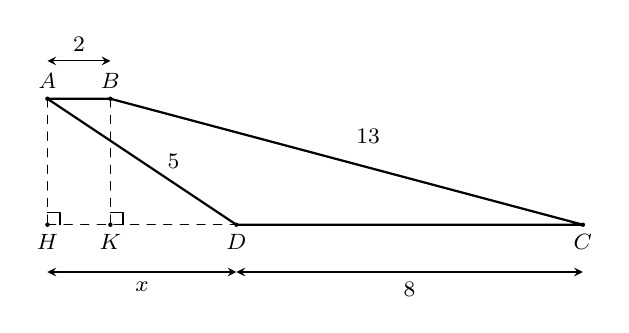
\begin{tikzpicture}[scale=0.4, font=\footnotesize, line join=round, line cap=round, >=stealth]
			\coordinate (H) at (0,0);
			\coordinate (A) at (0,4);
			\coordinate (D) at (6,0);
			\coordinate (C) at (17,0);
			\coordinate (B) at (2,4);
			\coordinate (K) at (2,0);
			\draw[thick] (A) -- (B) -- (C) -- (D) -- cycle;
			\draw[dashed] (A) -- (H);
			\draw[dashed] (B) -- (K);
			\draw[dashed] (H) -- (D);
			% Ký hiệu góc vuông tại H và K [cite: 2232]
			\draw (0,0.4) -- (0.4,0.4) -- (0.4,0);
			\draw (2,0.4) -- (2.4,0.4) -- (2.4,0);
			% Đánh dấu các điểm [cite: 718]
			\foreach \p/\pos in {A/above, B/above, C/below, D/below, H/below, K/below}
			\fill (\p) circle (2pt) node[\pos] {$\p$};
			% Ghi chú kích thước và tỉ lệ
			\draw[<->] (0,5.2) -- node[above] {$2$} (2,5.2); % Độ dài AB = 2
			\draw[<->] (6,-1.5) -- node[below] {$8$} (17,-1.5); % Độ dài CD = 8
			\draw[<->] (0,-1.5) -- node[below] {$x$} (6,-1.5); % Độ dài DH = x (vùng x âm)
			% Nhãn các cạnh theo giả thiết bài toán
			\node at (4.5,2) [left] {$5$};   % Cạnh AD = 5
			\node at (9.5,2.8) [right] {$13$}; % Cạnh BC = 13
		\end{tikzpicture}
	\end{center}
	\begin{itemchoice}
		\itemch Vì $H$ nằm trên đường thẳng $CD$ và $CD=8$, nên $CH = CD + DH =8 + x$.
		\itemch Trong tam giác vuông $ADH$,ta có $AH^2 = AD^2 - DH^2 = 5^2 - x^2 = 25 - x^2$,\\nên $AH=\sqrt{25-x^2}$.
		\itemch Kẻ $BK \perp CD$ tại $K$.\\ Vì $AB \parallel CD$ nên $ABKH$ là hình chữ nhật, suy ra $HK = AB = 2$. \\
		Khi đó $CK = CD + DH - HK = 8+ x-2=6 +x$. \\
		Trong tam giác vuông $BCK$, ta có $BK^2 = BC^2 - CK^2 = 13^2-(6 + x)^2=133-12x-x^2$,\\suy ra $BK=\sqrt{133-12x-x^2}$.\\
		Vì $AH=BK\Leftrightarrow \sqrt{25 - x^2} = \sqrt{133-12x-x^2}$.
		\itemch Giải phương trình $\sqrt{25 - x^2} = \sqrt{133-12x-x^2}$, ta có\\$25 - x^2 = 133- 12x - x^2 \Leftrightarrow 25 - x^2 = 133 + 12x - x^2 \Leftrightarrow 12x = 108 \Leftrightarrow x =9$.
	\end{itemchoice}
	}
\end{ex}
\Closesolutionfile{ans}
% \indapan{3}{ans/ans-c1b1-ds}
%---------------Trắc nghiệm trả lời ngắn
\ind{PHẦN III.} \inden{Câu trả lời ngắn.}
\setcounter{ex}{0}
\Opensolutionfile{ans}[ans/ans-c1b1-kq]

\begin{ex}%[0D7H3-2]
	Tính tích các nghiệm của phương trình $\sqrt{2x^2-9x+11}=x-1$ bằng.
	\shortans[oly]{$10$}
\loigiai{
	Bình phương hai vế của phương trình ta được
	$$2x^2-9x+11 = (x-1)^2 \Leftrightarrow 2x^2-9x+11 = x^2-2x+1 \Leftrightarrow x^2-7x+10=0.$$
	Giải phương trình bậc hai trên ta tìm được các giá trị là $x=2$ hoặc $x=5$.\\
	Thử lại các giá trị tìm được vào phương trình ban đầu
	\begin{itemize}
		\item Với $x=2$, ta có $\sqrt{2 \cdot 2^2 - 9 \cdot 2 + 11} = \sqrt{1} = 1$ (thỏa mãn).
		\item Với $x=5$, ta có $\sqrt{2 \cdot 5^2 - 9 \cdot 5 + 11} = \sqrt{16} = 4$ (thỏa mãn).
	\end{itemize}
	Phương trình đã cho có hai nghiệm phân biệt là $x=2$ và $x=5$.\\
	Vậy tích các nghiệm của phương trình là $2 \cdot 5 = 10$.
	}
\end{ex}
\begin{ex}%[0D7H3-1]% Câu 2
	Tổng các nghiệm của phương trình $\sqrt{3x^2-4x-1}=\sqrt{2x^2-2x+2}$ bằng.
	\shortans[oly]{$2$}
\loigiai{
	Bình phương hai vế của phương trình ta được
	\begin{align*}
		&3x^2-4x-1 = 2x^2-2x+2 \\
		\Leftrightarrow &x^2-2x-3=0 \\
		\Leftrightarrow &\hoac{ &x=3 \\ &x=-1.}
	\end{align*}
	Thử lại các giá trị tìm được vào phương trình ban đầu ta được:
	\begin{itemize}
		\item Với $x=3$, ta có $\sqrt{3 \cdot 3^2 - 4 \cdot 3 - 1} = \sqrt{14}$ và $\sqrt{2 \cdot 3^2 - 2 \cdot 3 + 2} = \sqrt{14}$ (thỏa mãn).
		\item Với $x=-1$, ta có $\sqrt{3(-1)^2 - 4(-1) - 1} = \sqrt{6}$ và $\sqrt{2(-1)^2 - 2(-1) + 2} = \sqrt{6}$ (thỏa mãn).
	\end{itemize}
	Phương trình đã cho có hai nghiệm phân biệt là $x_1 = 3$ và $x_2 = -1$.\\
	Vậy tổng các nghiệm của phương trình là $3 + (-1) = 2$.
	}
\end{ex}
\begin{ex}%[0D7H3-1]
	Gọi $S$ là tập nghiệm của phương trình $\sqrt{2x^2-3x-1}=\sqrt{x^2+x+4}$. Tính tổng các phần tử của tập hợp $S$.
	\shortans[oly]{$4$}
\loigiai{
	Bình phương hai vế của phương trình ta được
	$$2x^2-3x-1 = x^2+x+4 \Leftrightarrow x^2-4x-5=0 \Leftrightarrow \hoac{&x=-1\\&x=5.}$$
	Thử lại các giá trị tìm được vào phương trình ban đầu.
	\begin{itemize}
		\item Với $x=-1$, ta có $\sqrt{2(-1)^2-3(-1)-1} = \sqrt{4}=2$ và $\sqrt{(-1)^2+(-1)+4} = \sqrt{4}=2$ (thỏa mãn).
		\item Với $x=5$, ta có $\sqrt{2(5)^2-3(5)-1} = \sqrt{34}$ và $\sqrt{(5)^2+5+4} = \sqrt{34}$ (thỏa mãn).
	\end{itemize}
	Vậy tập nghiệm $S = \{-1; 5\}$.\\ Tổng các phần tử của tập hợp $S$ bằng $-1 + 5 = 4$.}
\end{ex}
\begin{ex}%[0D7V3-6]
	Một chiếc tàu thủy rời cảng $A$ chuyển động thẳng theo hướng Đông với vận tốc $20$ km/h. Cùng lúc đó, một canô rời cảng $B$ cách cảng $A$ là $10$ km về hướng Bắc, chuyển động thẳng về hướng Nam với vận tốc $40$ km/h. Giả sử tại thời điểm $t$ (giờ), khoảng cách giữa tàu thủy và canô được mô hình hóa bởi công thức $d = \sqrt{(20t)^2 + (10-40t)^2}$ (km). Hỏi sau mấy giờ kể từ khi xuất phát thì khoảng cách giữa tàu và canô bằng đúng khoảng cách từ cảng $B$ đến cảng $A$?
	\shortans[oly]{$0{,}4$}
\loigiai{
	Khoảng cách giữa cảng $A$ và cảng $B$ ban đầu là $10$ km.\\ Theo yêu cầu bài toán, ta có phương trình
	$$\sqrt{(20t)^2 + (10-40t)^2} = 10$$
	Bình phương hai vế của phương trình ($10 > 0$), ta được
	\begin{align*}
		&400t^2 + (10 - 40t)^2 = 100 \\
		\Leftrightarrow &400t^2 + 100 - 800t + 1\,600t^2 = 100 \\
		\Leftrightarrow &2\,000t^2 - 800t = 0 \\
		\Leftrightarrow &\hoac{ &t = 0 \\ &t = 0{,}4.}
	\end{align*}
	Vì ta xét thời điểm sau khi xuất phát nên $t = 0{,}4$ giờ (tức $24$ phút).\\
	Thử lại vào phương trình gốc, ta thấy $t=0{,}4$ thỏa mãn.\\
	Vậy sau $0{,}4$ giờ thì khoảng cách giữa hai tàu bằng $10$ km.
	}
\end{ex}
\begin{ex}%[0D7V3-6]
	Một cơ sở sản xuất đồ thủ công mỹ nghệ ước tính chi phí để sản xuất $x$ đơn vị sản phẩm (tính bằng triệu đồng) là $C(x) = \sqrt{3x^2 + 21x + 37}$. Doanh thu khi bán hết số sản phẩm đó là $R(x) = 2x + 5$ (triệu đồng). Để doanh nghiệp đạt trạng thái hòa vốn thì cơ sở cần sản xuất bao nhiêu đơn vị sản phẩm?
	\shortans[oly]{$4$}
\loigiai{
	Để doanh nghiệp hòa vốn, doanh thu phải bằng chi phí sản xuất, hay $C(x) = R(x)$.
	Ta có phương trình
	$$\sqrt{3x^2 + 21x + 37} = 2x + 5$$
	Điều kiện $x>0$.\\
	Bình phương hai vế của phương trình, ta được
	\begin{align*}
		&3x^2 + 21x + 37 = (2x + 5)^2 \\
		\Leftrightarrow &3x^2 + 21x + 37 = 4x^2 + 20x + 25 \\
		\Leftrightarrow &x^2 - x - 12 = 0 \\
		\Leftrightarrow &\hoac{&x = 4 \text{ (thỏa mãn)} \\ &x = -3 \text{ (loại).}}
	\end{align*}
	Vì số lượng sản phẩm $x$ phải là số dương nên ta chọn $x = 4$.\\
	Vậy để hòa vốn, cơ sở cần sản xuất $4$ đơn vị sản phẩm.
	}
\end{ex}
\begin{ex}%[0D7V3-6]
	Một trạm quan sát khí tượng $A$ đặt tại tọa độ $(0;3)$ trong hệ trục tọa độ $Oxy$ (đơn vị trên các trục là km). Một cơn bão đang di chuyển trên một con đường thẳng có phương trình $d\colon y = x - 1$. Một thiết bị quét của trạm $A$ chỉ có thể ghi nhận dữ liệu chính xác khi khoảng cách từ trạm đến tâm bão (điểm $M \in d$) bằng đúng quãng đường tâm bão đã di chuyển được tính từ điểm $M_0(1;0)$ trên đường thẳng $d$. Gọi tọa độ điểm $M(x;y)$ mà tại đó thiết bị bắt đầu ghi nhận dữ liệu, biết $x > 1$. Tính $x+y$.
	\shortans[oly]{$6$}
\loigiai{
	Gọi tọa độ tâm bão là $M(x; x-1) \in d$ với $x > 1$.\\
	Khoảng cách từ trạm $A(0;3)$ đến tâm bão $M$ là
	$$AM = \sqrt{(x-0)^2 + (x-1-3)^2} = \sqrt{x^2 + (x-4)^2} = \sqrt{2x^2 - 8x + 16}.$$
	Quãng đường tâm bão di chuyển từ $M_0(1;0)$ đến $M(x; x-1)$ là
	$$M_0M = \sqrt{(x-1)^2 + (x-1-0)^2} = \sqrt{2(x-1)^2} = \sqrt{2}\left|x-1\right|.$$
	Theo giả thiết $AM = M_0M$, ta có phương trình
	$$\sqrt{2x^2 - 8x + 16} = \sqrt{2}(x-1).$$
	Bình phương hai vế ($x>1$ nên vế phải dương)
	\begin{align*}
		&2x^2 - 8x + 16 = 2(x-1)^2 \\
		\Leftrightarrow &2x^2 - 8x + 16 = 2(x^2 - 2x + 1) \\
		\Leftrightarrow &2x^2 - 8x + 16 = 2x^2 - 4x + 2 \\
		\Leftrightarrow &4x = 14 \Leftrightarrow x = 3{,}5.
	\end{align*}
	Khi đó $y = x - 1 = 2{,}5$. \\
	Thử lại với $x=3{,}5$, $AM = \sqrt{2(3{,}5)^2 - 8(3{,}5) + 16} = \sqrt{24{,}5 - 28 + 16} = \sqrt{12{,}5} = 2{,}5\sqrt{2}$.\\
	$M_0M = \sqrt{2}(3{,}5-1) = 2{,}5\sqrt{2}$. thỏa mãn.\\
	Nên tọa độ điểm cần tìm là $M(3{,}5 ; 2{,}5)$.\\
	Suy ra $x=3{,}5$; $y=2{,}5$.\\
	Vậy $x+y=3{,}5+2{,}5=6$.
	}
\end{ex}
\Opensolutionfile{ans}[ans/ans-c1b1-kq]
\Closesolutionfile{ans}
% \indapan{4}{ans/ans-c1b1-kq}
%------------------Tự luận
\ind{PHẦN IV.} \inden{Tự luận.}
\setcounter{ex}{0}
\begin{ex}%[0D7H3-1]
	Tính tổng các nghiệm của phương trình $\sqrt{x^2 - 5x + 4} = \sqrt{x - 1}$.
\loigiai{
	Bình phương hai vế của phương trình, ta được
	\begin{align*}
		&x^2 - 5x + 4 = x - 1 \\
		\Leftrightarrow &x^2 - 6x + 5 = 0 \\
		\Leftrightarrow &\hoac{&x = 1 \\ &x = 5.}.
	\end{align*}
	Thử lại các giá trị tìm được vào phương trình $\sqrt{x^2 - 5x + 4} = \sqrt{x - 1}$.
	\begin{itemize}
		\item Với $x = 1$ ta có $\sqrt{1^2-5\cdot 1+4}=\sqrt{1-1}$. (thỏa mãn).
		\item Với $x = 5$ ta có $\sqrt{5^2-5\cdot 5+4}=\sqrt{5-1}$. (thỏa mãn).
	\end{itemize}
	Vậy phương trình có hai nghiệm $x_1 = 1, x_2 = 5$. Tổng các nghiệm là $1 + 5 = 6$.
	}
\end{ex}
\begin{ex}%[0D7H3-2]%Câu 2 TL
	Giải phương trình $\sqrt{2x^2 - 3x + 1} = x - 1$.
\loigiai{
	Bình phương hai vế của phương trình, ta được
	\begin{align*}
		&2x^2 - 3x + 1 = (x - 1)^2 \\
		\Leftrightarrow &2x^2 - 3x + 1 = x^2 - 2x + 1 \\
		\Leftrightarrow &x^2 - x = 0 \\
		\Leftrightarrow &\hoac{ &x = 0 \\ &x = 1.}
	\end{align*}
	Thử lại vào phương trình ban đầu ta được
	\begin{itemize}
		\item Với $x = 0$ ta có vế phải bằng $0 - 1 = -1 < 0$. (loại).
		\item Với $x = 1$ ta có  $\sqrt{2\cdot 1^2 - 3\cdot 1 + 1} = 0$. (thỏa mãn).
	\end{itemize}
	Vậy phương trình có nghiệm duy nhất $x = 1$.
	}
\end{ex}
\begin{ex}%[0D7H3-2]% Câu 3 TL
	Cho phương trình $\sqrt{3x^2 - 9x + 7} = x - 1$. Tính giá trị của biểu thức $S = 4x_1 + x_2$, trong đó $x_1> x_2$ là các nghiệm của phương trình đã cho.
\loigiai{
	Bình phương hai vế của phương trình, ta được:
	\begin{align*}
		&3x^2 - 9x + 7 = (x - 1)^2 \\
		\Leftrightarrow &3x^2 - 9x + 7 = x^2 - 2x + 1 \\
		\Leftrightarrow &2x^2 - 7x + 6 = 0\\
		\Rightarrow& \hoac{ &x = 2 \\ &x = 1{,}5.}
	\end{align*}
	Thử lại
	\begin{itemize}
		\item Với $x = 2$ ta có $\sqrt{3\cdot 2^2 - 9\cdot 2 + 7} = 2 - 1$. (thỏa mãn).
		\item Với $x = 1{,}5$ ta có $\sqrt{3\cdot (1{,}5)^2 - 9\cdot 1{,}5 + 7} = 1{,}5 - 1$. (thỏa mãn).
	\end{itemize}
	Vậy phương trình có hai nghiệm $x_1 = 2$ và $x_2 = 1{,}5$.\\
	Giá trị của biểu thức $S = 2 + 1{,}5 = 3{,}5$.
	}
\end{ex}
\begin{ex}%[0D7V3-6]
	Một mảnh vườn hình tam giác vuông có hai cạnh góc vuông lần lượt là $2x$ (m) và $x+1$ (m). Biết cạnh huyền của tam giác đó dài $\sqrt{x^2 + 13x + 4}$ (m). Tìm giá trị của $x$.
\loigiai{
	\begin{center}
		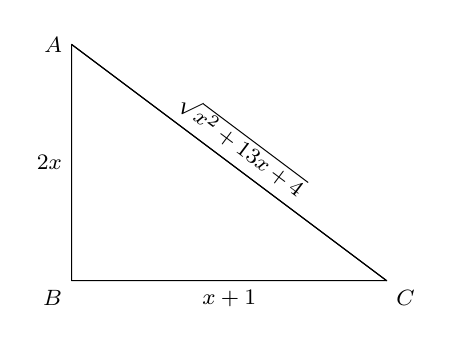
\begin{tikzpicture}[scale=1, font=\footnotesize, line join=round, line cap=round, >=stealth]
			\coordinate (B) at (0,0);
			\coordinate (C) at (4,0);
			\coordinate (A) at (0,3);
			\draw (A) -- (B) -- (C) -- cycle;
			\tkzMarkRightAngle[size=0.3](A,B,C)
			\node[left] at (0,1.5) {$2x$};
			\node[below] at (2,0) {$x+1$};
			\draw (A) -- (C) node[midway, sloped, above] {$\sqrt{x^2 + 13x + 4}$};
			\node[left] at (A) {$A$};
			\node[below left] at (B) {$B$};
			\node[below right] at (C) {$C$};
		\end{tikzpicture}
	\end{center}
	Điều kiện  $x> 0$.\\
	Theo định lý Pitago, ta có phương trình
	\begin{align*}
		&(2x)^2 + (x+1)^2 = \left(\sqrt{x^2 + 13x + 4}\right)^2 \\
		\Leftrightarrow &4x^2 + x^2 + 2x + 1 = x^2 + 13x + 4 \\
		\Leftrightarrow &5x^2 + 2x + 1 = 2x^2 + 10x + 1 \\
		\Leftrightarrow &4x^2 - 11x -3= 0 \\
		\Leftrightarrow &\hoac{&x =-\dfrac{1}{4} \text{ (loại)} \\ &x = 3 \text{ (thỏa mãn)}.}
	\end{align*}
	Vậy giá trị cần tìm là $x=3$.
	}
\end{ex}
\begin{ex}%[0D7C3-6]
	Một trạm biến áp được xây dựng tại đảo $A$ cách bờ biển một khoảng $AH = 4$ km. Người ta dự định kéo đường dây điện từ đảo $A$ đến vị trí $M$ trên bờ biển, rồi từ $M$ kéo thẳng đến trạm phân phối $B$ nằm trên đất liền (như hình vẽ). Biết trạm $B$ cách hình chiếu $H$ một khoảng $HB = 9{,}25$ km. Chi phí lắp đặt mỗi km dây điện dưới nước là $5$ triệu đồng, chi phí trên bờ là $4$ triệu đồng. Biết rằng tổng chi phí lắp đặt trên biển và trên bờ là bằng nhau. Tính khoảng cách $x = HM$ (km).
\loigiai{
	\begin{center}
		\begin{tikzpicture}[>=stealth, scale=0.8, font=\footnotesize]
			% Định nghĩa các điểm
			\path
			(0,4) coordinate (A)
			(0,0) coordinate (H)
			(3,0) coordinate (M)
			(9.25,0) coordinate (B);
			% Vẽ mặt biển và bờ biển
			\fill[blue!10] (-1,0) rectangle (10,4);
			\fill[brown!20] (-1,-1) rectangle (10,0);
			\draw[thick] (-1,4) -- (10,4);
			\draw[thick, brown!50!black] (-1,0) -- (10,0);
			% Vẽ các đoạn thẳng liên kết
			\draw[blue, thick] (A) -- (M); % Đường dây dưới nước
			\draw[red, thick] (M) -- (B); % Đường dây trên bờ
			\draw[dashed] (A) -- (H) -- (M);
			% Vẽ ký hiệu góc vuông tại H
			\draw (0,0.3) -- (0.3,0.3) -- (0.3,0);
			% Hiển thị các điểm
			\foreach \p/\pos in {A/above, H/below left, M/below, B/below}
			\fill (\p) circle (1.5pt) node[\pos] {$\p$};
			% Ghi chú kích thước
			\draw[<->] (-0.5,0) -- node[left] {$4$ km} (-0.5,4);
			\draw[<->] (0,-0.8) -- node[below] {$x$} (3,-0.8);
			\draw[<->] (3,-0.8) -- node[below] {$9{,}25 - x$} (9.25,-0.8);
			% Nhãn
			\node at (5,2) {\textbf{BIỂN}};
			\node at (5,-0.5) {\textbf{ĐẤT LIỀN}};
		\end{tikzpicture}
	\end{center}
	Quãng đường dây điện dưới nước là $AM = \sqrt{x^2 + 4^2} = \sqrt{x^2 + 16}$ (km).\\
	Quãng đường dây điện trên bờ là $MB = 9{,}25 - x$ (km).\\
	Chi phí lắp đặt dưới nước là $5\sqrt{x^2 + 16}$ (triệu đồng).\\
	Chi phí lắp đặt trên bờ là $4(9{,}25 - x)$ (triệu đồng).\\
	Theo đề bài, tổng chi phí dưới nước bằng tổng chi phí trên bờ nên ta có phương trình
	$$5\sqrt{x^2 + 16} = 4(9{,}25 - x) \Leftrightarrow 5\sqrt{x^2 + 16} = 37 - 4x.$$
	Điều kiện: $37 - 4x \ge 0 \Leftrightarrow x \le 9{,}25$.\\
	Bình phương hai vế của phương trình, ta được
	\begin{align*}
		&25(x^2 + 16) = (37 - 4x)^2 \\
		\Leftrightarrow &25x^2 + 400 = 1369 - 296x + 16x^2 \\
		\Leftrightarrow &9x^2 + 296x - 969 = 0\\
		\Leftrightarrow &\left[\begin{aligned} &x=3 \quad \text{(thỏa mãn)} \\ &x=-\dfrac{323}{9} \quad \text{(loại).} \end{aligned} \right.
	\end{align*}
	Vậy khoảng cách $HM$ cần tìm là $x = 3$ km.
	}
\end{ex}
\begin{ex}%[0D7V3-6]
	Một công ty dự định sản xuất một loại sản phẩm mới. Chi phí cố định để thiết lập dây chuyền là $100$ triệu đồng. Chi phí để sản xuất $x$ sản phẩm được cho bởi công thức $C(x) = \sqrt{x^2 + 400x + 40\,000}$ (triệu đồng). Giá bán mỗi sản phẩm là $1{,}2$ triệu đồng. Gọi $x$ là số sản phẩm cần sản xuất để công ty đạt được lợi nhuận là $200$ triệu đồng. Tính số sản phẩm $x$ cần sản xuất.
\loigiai{
	Doanh thu từ việc bán $x$ sản phẩm là $T(x) = 1{,}2x$ (triệu đồng).\\
	Tổng chi phí sản xuất là $C'(x) = 100 + \sqrt{x^2 + 400x + 40\,000}$ (triệu đồng).\\
	Lợi nhuận được tính bằng $L(x)=T(x)-C'(x)$.
	\begin{align*}
		L(x) =& 1{,}2x - \left(100 + \sqrt{x^2 + 400x + 40\,000}\right) = 200.\\
		\Leftrightarrow& \sqrt{x^2 + 400x + 40\,000} = 1{,}2x - 300. (*)
	\end{align*}
	Bình phương hai vế
	\begin{align*}
		&x^2 + 400x + 40\,000 = (1{,}2x - 300)^2 \\
		\Leftrightarrow &x^2 + 400x + 40\,000 = 1{,}44x^2 - 720x + 90\,000 \\
		\Leftrightarrow &0{,}44x^2 - 1120x + 50\,000 = 0\\
		\Leftrightarrow &\hoac{&x=2\,500\\&x=\approx 45{,}45\; \text{(loại)}.}
	\end{align*}
	Thử lại ta có\\
	Với $x=2500$ thay vào phương trình (*) $\sqrt{(2500)^2+400\cdot2\,500+40\,00}=1{,}2\cdot2\,500-300=2\,700$ (thỏa mãn).\\
	Với $x=45,45$ thì vế phải phương trình (*) bằng $-245{,}46<0$ (loại).\\
	Vậy $x = 2500$ (sản phẩm).
	}
\end{ex}
\Closesolutionfile{ans}